%\documentclass[preprint]{acm_proc_article-sp}
\documentclass{sig-alternate}

%\usepackage{latexsym}
%\usepackage{times}
\usepackage{graphicx}
\usepackage{subfigure}
\usepackage{color}
\usepackage{amsmath,amssymb}
\usepackage{algorithm,algorithmic}
\usepackage{url}


\newcommand{\id}[1]{\ensuremath{#1}}
\newtheorem{example}{Example}

\title{Performance Evaluation of WattDepot Using Various Database Backends}

\numberofauthors{1}
\author{
      \alignauthor George Lee\\
       \affaddr{University of Hawai`i at M\={a}noa}\\
       \affaddr{Honolulu, HI 96822, USA}\\
       \email{\normalsize{gelee@hawaii.edu}}
}


\begin{document}

\maketitle

\begin{abstract}
Investigating ``smart grid'' uses and technologies is a new and popular area of research.  Investigating how people both use energy and how they respond to feedback about their use can help researchers figure out ways to help people save energy.  One such tool for collecting and/or simulating energy use is ``WattDepot'', developed here at the University of Hawai`i at M\={a}noa.  Because most of the data stored by WattDepot is energy/power data, the data storage backend does not necessarily need to be a traditional relational database.  We implemented two non-relational database backends, Berkeley DB Java Edition and Mongo DB, and designed benchmarks to evaluate their performance.  As a result of the benchmarks, we found that the non-relational database backends outperformed the existing relational database backend by as much as 65 percent.
\end{abstract}

\section{Introduction}

Collecting and analyzing energy data is one of the up and coming areas of research.  Because of our limited resources and the rising costs of energy, figuring out ways to change people's energy behavior is becoming increasingly important.  Providing feedback to residents about their energy usage in their own homes and apartments is one way to get people to change their behavior.  If residents can see their energy use on a much more granular scale, they can begin to figure out why their costs are so high.

Seeing as how this is a popular area of research, it is not surprising that several organizations have come up with systems for providing some level of feedback.  One solution developed here at the University of Hawaii at M\={a}noa is WattDepot\cite{wattdepot}; an open source web service that collects and stores electricity data.  Clients are then able to query this web service in order to analyze the data or provide visualizations.

WattDepot is an integral part of an upcoming residence hall energy competition here at the University of Hawaii at M\={a}noa called the Kukui Cup.  In this competition, 4 buildings with 10 meters each will be sending data to a WattDepot server on 15 second intervals.  This near real-time data will then be presented on a web application developed for the competition based on Makahiki\cite{makahiki}; a web application framework for energy competitions.  Thus, it is critical that WattDepot stores its data as efficiently as possible while making it available to be queried at the same time.

While WattDepot is set up to support various database backends, it currently uses Apache Derby\cite{apachederby}; a relational database for Java.  Given that most of the data that will be used is energy data, we want to investigate non-relational data storage solutions to see if they provide a significant performance boost compared to the existing relational database.  We also want to see how well they integrate with the existing WattDepot architecture.  We chose two non-relational data storage systems; Berkeley DB Java Edition and MongoDB.

The rest of this paper is as follows: Section \ref{sec:background} will provide some background of WattDepot and the database systems involved in the benchmark experiment.  Section \ref{sec:benchmark} will outline the design of the benchmarks and how they match up to real-world use of WattDepot.  Section \ref{sec:experiments} will provide the results of the benchmarks and some analysis  Finally, Section \ref{sec:conclusion} goes into the implications of the results and future work that needs to be done.

\section{Background}
\label{sec:background}

This section will go over WattDepot and the various backends we will be using.  Section \ref{sub:wattdepot} will provide some information on WattDepot and how its architecture makes it possible to use both relational and non-relational database backends.  Sections \ref{sub:derby}, \ref{sub:Berkeley DB Java Edition}, and \ref{sub:mongodb} will give some background information on Derby, Berkeley DB Java Edition, and MongoDB respectively.

\subsection{WattDepot}
\label{sub:wattdepot}

WattDepot is an open source web service that collects energy and power data and stores that information into a database.  The database can also be queried in order to generate visualizations or perform analyses on the data.  WattDepot can be used to simulate data and facilitate experimentation when developing ``Smart Grid'' applications.

The WattDepot website states that it ``is architecturally decoupled from the underlying storage technology''.  In essence, this means that WattDepot is flexible enough to support various database backends.  This includes non-relational database management systems as well as the traditional relational database management systems.  This is possible due to the relatively simple data architecture used by WattDepot.  First, there are only three types of entities in WattDepot; Users, Sources, and Sensor Data.  Users are used to authenticate to the server via the REST API.  Simple access controls are available to prevent unauthorized users from creating/deleting entities.  Sources represent sources of data in WattDepot.  Note that this is not to be confused with energy sources; consumers of energy are also sources within the system.  The names of these Sources are used in Sensor Data to identify where the data originated from.  Sensor Data are raw readings received from the various sources.  Sensor Data can contain information about energy generated/consumed and/or power generated/consumed.  Sensor Data also may contain information about the carbon emissions of this Source.

In terms of the number of rows, Sensor Data dominates the other entities in WattDepot.  Take for example the Kukui Cup, our upcoming energy competition. In this competition, we plan to have 4 towers with 10 meters each sending data every 15 seconds.  Each meter would then create 5,760 rows of Sensor Data in a day.  In total, these 40 Sources will create 230,400 rows of Sensor Data every day.  Furthermore, this data must be queried by the competition's website, which will be used by hundreds of students living in the residence halls.

However, once we know the names of the sources (which is unlikely to change), we rarely have to look at Users and Sources.  This also means that joins are not required, as we are mostly looking at collections of Sensor Data.  While such a system can be implemented using relational databases, this situation is perfect for non-relational database systems like Berkeley DB Java Edition or NoSQL solutions.  Because a relational database system (Derby) is currently used in WattDepot, the next step is to implement non-relational database systems and compare them to the existing system in terms of performance.

\subsection{Derby}
\label{sub:derby}

Apache Derby is a relational database system written entirely in Java.  Initially developed by Cloudscape Derby is also known as JavaDB, which is included in java 1.6.  The goal of Derby is to be portable, embeddable, and have a small footprint while being SQL and JDBC compliant.  Furthermore, because it is pure Java, it runs on any platform with a JVM with little effort.  The Apache Derby Wiki\cite{derby-wiki} contains documentation as well as details on the internals of Derby.

Because WattDepot is developed using Java, using Derby is a natural choice.  Not only is it readily available, but it is easily accessible using JDBC.  Additionally, because it can be used in an embedded mode, it reduces the amount of system administration needed to maintain a client/server database system.

\subsection{Berkeley DB Java Edition}
\label{sub:Berkeley DB Java Edition}

Oracle Berkeley DB is a lightweight, high-performance embedded database for key/value data.  Berkeley DB is not a relational database\cite{berkeley-isnt} and does not support SQL queries. Oracle provides three different Berkeley DB products; Berkeley DB, Berkeley DB Java Edition, and Berkeley DB XML.

Berkeley DB Java Edition is a pure Java database that replicates most of the functionality of the main Berkeley DB product.  While it is not JDBC compliant (because it does not support SQL), objects can be persisted using the Java Collections API.  The Berkeley DB Java Edition Data Sheet\cite{berkeleydb-datasheet} also notes that the lack of SQL processing dramatically improves performance.  As a result of the way data is stored and retrieved in WattDepot, we have little need for the ``relational'' features of SQL like joins.  This makes BerkeleyDB a very good fit for WattDepot.

\subsection{MongoDB}
\label{sub:mongodb}

MongoDB\cite{mongodb} is a scalable, open source NoSQL database written in C++.  Instead of using the traditional rows in tables that relational databases use, MongoDB uses JSON style documents that have flexible schemas.  MongoDB has become one of the more popular NoSQL solutions and is used by companies and organizations such as Intuit, SourceForge, CERN, and more\cite{mongodb-deployments}.

Unlike Derby and Berkeley DB Java Edition, Mongo DB is a client/server database and is not available as an embedded database.  In addition, it is not implemented in Java, although client drivers for various different programming languages are available.  On the other hand, it is also ideal for WattDepot because there is no need for SQL joins

\section{Benchmark Design}
\label{sec:benchmark}

After implementing the methods required by WattDepot for storing and retrieving data for both Berkeley DB Java Edition and MongoDB, we developed benchmarks to compare the performance of these new implementations with the existing Derby implementation.  We implemented benchmarks that operate directly with the server API rather than using the REST client API.  The three different benchmarks are inserts, random single data query, and random daily data query.

To benchmark the inserts, we inserted 1,000,000 rows of sensor data into the database.  The rows are inserted sequentially and correspond to sensor data for a single source taken every 15 seconds.  Because data from many sources can be inserting data all at once, this benchmark is designed to observe the amount of time it takes on average to insert a row of sensor data.  We also used 1,000,000 rows because this data will also be used for the other two benchmarks.

The next two benchmarks are random queries.  First, we randomly retrieved a single row of sensor data from the database 1,000 times to observe each implementation's random read performance.  Random reads can happen in the real world when WattDepot needs to use data interpolation.  When a client queries WattDepot for energy/power data, data may not exist precisely at that time.  In order to handle this situation, the server calculates a ``data straddle'', which consists of the first data point before that point in time and the first data point after that point in time.  The server calculates the difference between the two and uses that to provide a result to the user.

The other random query benchmark consists of selecting sensor data for a random 24 hour period.  Because the simulated data is taken at a 15 second interval, this benchmark randomly retrieves blocks of 5,760 rows of sensor data.  This benchmark evaluates the implementation's ability retrieve daily information.  Since energy is power multiplied by time, this query can be used to calculate the amount of energy generated/consumed by the source over the last 24 hours.

Each of the above benchmarks are designed to be executed both serially and in parallel.  The parallel benchmarks represent a more ``real-world'' environment where various sensors and clients may be querying the server.  For the parallel insertion benchmark, the 1,000,000 rows of sensor data are divided between the available threads.  For example, if there are 2 threads, then each thread will insert 500,000 rows of sensor data.  The load of the query benchmarks are also divided by the number of threads.  By default, each of the query benchmarks query the server 1,000 times.  Thus, if there are two threads, then each thread will query the database 500 times.

\begin{figure*}
	\centering
	\subfigure[Serial Insertions]
	{
		\label{exp:serial-inserts}
		\includegraphics[width=8cm]{images/serial-insertions.eps}
	}
	\hspace{1cm}
	\subfigure[Parallel Insertions]
	{
		\label{exp:parallel-inserts}
		\includegraphics[width=8cm]{images/parallel-insertions.eps}
	}
	\hspace{1cm}
	\subfigure[Serial Random Single Data Query]
	{
		\label{exp:serial-single}
		\includegraphics[width=8cm]{images/serial-single-query.eps}
	}
	\hspace{1cm}
	\subfigure[Parallel Random Single Data Query]
	{
		\label{exp:parallel-single}
		\includegraphics[width=8cm]{images/parallel-single-query.eps}
	}
	\hspace{1cm}
	\subfigure[Serial Random Daily Query]
	{
		\label{exp:serial-daily}
		\includegraphics[width=8cm]{images/serial-daily-query.eps}
	}
	\hspace{1cm}
	\subfigure[Parallel Random Daily Query]
	{
		\label{exp:parallel-daily}
		\includegraphics[width=8cm]{images/parallel-daily-query.eps}
	}
	\caption{Experimental results (lower is better)}
	\label{exp:experimental-graphs}
\end{figure*}

\section{Experiments}
\label{sec:experiments}

The benchmarks in section \ref{sec:benchmark} were performed on a Macbook Pro with a 2.4 GHz dual core processor and 4 GB of memory using Java version 1.6.0.  We used version 4.1.7 of Berkeley DB Java Edition and version 1.8.1 of Mongo DB.  The benchmarks were run both serially and in parallel for each implementation.  The parallel benchmarks used 4 threads to execute the tasks.  We ran the insertion benchmark first before running the random queries.  Figure \ref{exp:experimental-graphs} shows the results of the benchmarks both serially and in parallel.

In all of the above graphs, both Berkeley DB and Mongo DB perform better than Derby.  In fact, Berkeley DB is the clear winner in all of them, outperforming Derby in the serial benchmarks by 64 percent in the serial insertions and random queries.  Mongo DB, while not quite as fast as Berkeley DB, still shows a 54 percent improvement in serial inserts over Derby.  On the other hand, Mongo DB shows modest improvements of 26 percent and 16 percent in the serial and daily benchmarks respectively.  

One thing to note is that figure \ref{exp:parallel-inserts} shows \emph{total} insertion time and not average insertion time and is also shown on log scale.  This is because Derby is about 100 times worse than both Berkeley DB and Mongo DB.  In fact, the total insertion time of Mongo DB and Berkeley DB are between 2 and 3 minutes, while Derby's total insertion time is about 3 hours and 45 minutes.  Once the data was inserted though, the query results were very similar to the serial benchmarks.  However, we do see some speed gains overall from having 4 threads, as Derby's query speed increased by about 40 percent in the single data query and 77 percent in the daily data query.  However, the performance gain was matched by Berkeley DB and Mongo DB, with Berkeley DB still outperforming Derby by about 65 percent.

Given the complicated nature of these database management systems and the limited time, it is difficult to figure out the reasons behind the benchmarks.  However, we can make a few guesses.  One reason for Derby's poor insertion performance may be reindexing after each insert into the database.  Thus, as the table gets larger, the reindexing may take more and more time.  In the future, we may want to investigate the time it takes Derby to recalculate the index or try doing a bulk load of data with indexes disabled until the load completes.  Mongo DB, which also uses indexes, may also be affected by this same issue.

In addition to the indexes, Mongo DB's insert performance may have been affected by ``write concerns''.  Normally, when a client inserts data into a Mongo DB collection, the operation returns right away without waiting for the response from the server.  This means that the operation always returned successfully unless there was a network issue.  However, to pass the WattDepot unit tests for database implementations, we needed to wait for the result from the server in order to see if the operation was successful or not.  This may further improve Mongo DB's insert performance, although the Mongo DB implementation really could use a query performance improvement.

While the Berkeley DB embedded database comes out ahead, it is important to note that in larger deployments, an embedded database may not be able to handle the same level of concurrency that a traditional client/server database system can handle.  However, since WattDepot is handling the client requests, this may not be as much of a concern.  Ultimately, because Mongo DB is a more proven solution in large deployments, the reliability of the server may be worth the relative performance costs.

\section{Conclusion}
\label{sec:conclusion}

Because WattDepot's architecture allows us to implement both relational and non-relational backends, it provided a perfect setting for comparing the performance of these backends.  In addition to the existing Derby implementation, we added a Berkeley DB implementation and a Mongo DB implementation.  We then designed benchmarks to approximate how WattDepot might query this data in the real world.  After running the benchmarks both serially and in parallel, we found that while both Berkeley DB and Mongo DB came out ahead of Derby, Berkeley DB showed significant performance gains.

However, the reasons behind these benchmarks were largely unanswered.  In the future, we could investigate inserting data into Derby and/or Mongo DB in bulk to see if reindexing is taking place and what kind of performance overhead does it have.  We also did little in the way of performance tuning these implementations.  Also, Mongo DB is not the only NoSQL solution.  Other popular NoSQL solutions include Redis, Riak, and Cassandra.  Perhaps one of these solutions can improve on Mongo DB and maybe even dethrone Berkeley DB as the performance champion.

\bibliographystyle{abbrv}
\bibliography{paper}

\end{document}

